\section{Целочисленное деление}
\label{ch:div:int}

В результате целочисленного деления числа $A$ (делимое) на число $d$ (делитель) получается частное $q$ и остаток $\Delta$, такие, что выполняется равенство:
\[
    A = q \cdot d + \Delta,
\]
где $A, q, d, \Delta$ --- целые числа.

При этом остаток всегда менше делителя по модулю:
\[
    |\Delta|<|d|.
\]

Так как в результате операции целочисленного деления определяется два числа: частное $q$ и остаток $\Delta$, то результат деления $A\div d$ будет записываться следующим образом:
\[
    A\div d=\DivAnswer{q}{\Delta},
\]
например: $7\div 3=\DivAnswer{2}{1}$.

Когда в делении участвуют отрицательные целые числа, то результат неоднозначен (всегда имеются два варианта), хотя общее правило $|\Delta|<|d|$ --- соблюдается.  Например, при делении $({-7})\div({-3})$ можно получить результат, равный как $\DivAnswer{2}{-1}$, так и $\DivAnswer{3}{2}$.

\begin{table}[!ht]
    \caption{Неоднозначность целочисленного деления}
    \label{t:div:int:undefined}
    \centering
    \begin{tabular}{lc||l|l|l}
        \hline\hline
        Пример        & &Отсечение          &\multicolumn{1}{|p{.22\textwidth}|}{Положительный модуль}
                                                               & \multicolumn{1}{p{.22\textwidth}}{Меньшее частное} \\
        \hline\hline
        $7\div 3$     &=&\DivAnswer{ 2}{1}  &\DivAnswer{ 2}{1} & \DivAnswer{ 2}{ 1} \\
        $(-7)\div 3$  &=&\DivAnswer{-2}{-1} &\DivAnswer{-3}{2} & \DivAnswer{-3}{ 2} \\
        $7\div(-3)$   &=&\DivAnswer{-2}{1}  &\DivAnswer{-2}{1} & \DivAnswer{-3}{-2} \\
        $(-7)\div(-3)$&=&\DivAnswer{ 2}{-1} &\DivAnswer{ 3}{2} & \DivAnswer{ 2}{-1} \\ \hline
    \end{tabular}
\end{table}
    
Чтобы гарантировать однозначность результатов, вводятся дополнительные ограничения на результат. Обычно используется одно из трех следующих правил.
\begin{itemize}
    \item \emph{Правило отсечения}. Из неоднозначных результатов выбирается верным результат с меньшим по модулю частным (или, что то же, в качестве частного фиксируется целая часть рационального деления).
    \item \emph{Правило положительного модуля}. Выбирается верным результат с положительным остатком.
    \item \emph{Правило меньшего частного}. Выбирается результат с меньшим из возможных частных.
\end{itemize}

Примеры однозначных результатов, полученных по данным правилам, приведены в таблице \ref{t:div:int:undefined}.

\begin{Note}
    Результат целочисленного деления, как обратной умножению операции, получается серией вычитаний и сдвигов.
\end{Note}

Современные языки программирования высокого уровня, используемые для системного программирования (а также и большинство современных процессоров) разделяют целочисленные типы на беззнаковые числа и числа со знаком. В соответствии с таким разделением, отдельно рассматриваются алгоритмы деления беззнаковых чисел и алгоритмы деления в дополнительном коде (т.е. числа со знаком).


\subsection{Беззнаковое деление}

В даннном разделе будет рассматриваться только деление положительных чисел --- чисел <<без знака>>. В этом случае и частное $q$ и остаток $\Delta$, совместно формирующие результат $\DivAnswer{q}{\Delta}$, должны быть положительны.

Рассмотрим на примере способ, которым учат делить нацело европейских школьников --- он чуть лучше отражает суть машинных способов, чем отечественный. Вначале рассмотрим пример в десятичной системе счисления, предполагая, что умножением мы уже владеем.

Пусть нужно разделить $53239$ на $223$. Заранее сообщаем результат:
\[
    53239\div 223 = \DivAnswer{238}{165}
\]

Теперь разберемся как его получить. Записываем в шапку будущей таблицы делитель и делимое, оставляя сверху над делителем место под частное. 
\[
    \begin{tabular}{cccccc|cl}
          \multicolumn{6}{c|}{\emph{\tiny Место под частное}} &  & Примечания\\ 
          \hline\hline
          & 5 & 3 & 2 & 3 & 9 & ${\div 223}$ &\\
          \hline\hline
    \end{tabular}
\]

На каждом шаге процесса деления будет определяться очередная цифра частного и записываться над соответствующей цифрой делителя. На первом шаге в первой стоке выписывается первая цифра делимого и рассматривается как число:
\[
    \begin{tabular}{cccccc|cl}
           
          &   &   &   &   &   &              & Примечания\\ 
          \hline\hline
          & 5 & 3 & 2 & 3 & 9 & ${\div 223}$ &\\
          \hline\hline
          & 5 &   &   &   &   &              &\\
    \end{tabular}
\]

$5$ меньше $223$ и определить первую цифру частного, записываемую над первой цифрой делимого, легко --- она равна нолю:
\(5\div 223 = \DivAnswer{0}{5}.\) 
\[
    \begin{tabular}{cccccc|cl}
           
          & 0 &   &   &   &   &              & Примечания\\ 
          \hline\hline
          & 5 & 3 & 2 & 3 & 9 & ${\div 223}$ &\\
          \hline\hline
          & 5 &   &   &   &   &              &$5\div 223 = \DivAnswer{0}{5}$\\ \hline
    \end{tabular}
\]

При этом в строке остается без изменений остаток первого шага: число $5$. На втором шаге, во второй строке к остатку первого шага дописывается вторая цифра делимого и подбирается вторая цифра частного: 
\[
    \begin{tabular}{cccccc|cl}
           
          & 0 & 0 &   &   &   &              & Примечания\\ 
          \hline\hline
          & 5 & 3 & 2 & 3 & 9 & ${\div 223}$ &\\
          \hline\hline
          & 5 &   &   &   &   &              & \\ \hline
          & 5 & 3 &   &   &   &              &$53\div 223 = \DivAnswer{0}{53}$ \\ \hline
          \\
    \end{tabular}
\]

На третьем шаге, к текущему остатку дописывается третья цифра делимого и подбором, наконец, удается найти первую значащую цифру частного:
\[
    \begin{tabular}{cccccc|cl}
           
          & 0 & 0 & 2 &   &   &              & Примечания\\ 
          \hline\hline
          & 5 & 3 & 2 & 3 & 9 & ${\div 223}$ &\\
          \hline\hline
          & 5 &   &   &   &   &              & \\ \hline
          & 5 & 3 &   &   &   &              & \\ \hline
          & 5 & 3 & 2 &   &   &              & $532\div 223 = \DivAnswer{2}{86}$ \\ 
        - & 4 & 4 & 6 &   &   &              & $223\cdot 2 = 446$ \\ \cline{2-4}
        = &   & 8 & 6 &   &   &              & $532-446 = 86$ \\ \hline
          \\
    \end{tabular}
\]

Таким образом процесс повторяется до последней цифры делимого, результаты расчетов приведены на рисунке \ref{t:div:int:decimalDiv}.
\begin{figure}[!ht]
    \centering
    \begin{tabular}{cccccc|cl}
           
          & 0 & 0 & 2 & 3 & 8 &              & Примечания\\ 
          \hline\hline
          & 5 & 3 & 2 & 3 & 9 & ${\div 223}$ &\\
          \hline\hline
          & 5 &   &   &   &   &              & $5\div 223 = \DivAnswer{0}{5}$   \\ \hline
          & 5 & 3 &   &   &   &              & $53\div 223 = \DivAnswer{0}{53}$ \\ \hline
          & 5 & 3 & 2 &   &   &              & $532\div 223 = \DivAnswer{2}{86}$ \\ 
        - & 4 & 4 & 6 &   &   &              & \\ \cline{2-4}
        = &   & 8 & 6 &   &   &              & \\ \hline
          &   & 8 & 6 & 3 &   &              & $863\div 223 = \DivAnswer{3}{194}$\\ 
        - &   & 6 & 6 & 9 &   &              & \\ \cline{3-5}
        = &   & 1 & 9 & 4 &   &              & \\ \hline
          &   & 1 & 9 & 4 & 9 &              & $1949\div 223 = \DivAnswer{8}{165}$\\ 
        - &   & 1 & 7 & 8 & 4 &              & \\ \cline{4-6}
        = &   &   & 1 & 6 & 5 &              & \\ \hline
          &   &   &   &   &   &              & Ответ: $53239\div 223 = \DivAnswer{238}{165}$ \\ 
          \\
    \end{tabular}
	
    \caption{$53239\div 223 = \DivAnswer{238}{165}$ в 10СС}
    \label{t:div:int:decimalDiv}
\end{figure}

На последнем шаге получены все цифры частного $q$ и окончательный остаток $\Delta$. 

Если в десятичной системе счисления на каждом шаге требуется подобрать очередную цифру частного из десяти вариантов, то в двоичной системе счисления все заметно упрощается: если текущий остаток меньше делителя, то цифра частного $0$, в противном случае $1$. Пример деления $33\div 5$ приводится на рисунке \ref{t:div:int:binaryDiv}.

\begin{table}[!ht]
    \caption{$33\div 5 = \DivAnswer{6}{3}$ в 2СС}
    \label{t:div:int:binaryDiv}
    \centering
    \begin{tabular}{ccccccc|cl}
           
          & 0 & 0 & 0 & 1 & 1 & 0 &              & \\ 
          \hline\hline
          & 1 & 0 & 0 & 0 & 0 & 1 & ${\div 101}$ & Примечания\\
          \hline\hline
          & 1 &   &   &   &   &   &              & $1<101$\\ \hline
          & 1 & 0 &   &   &   &   &              & $10<101$\\ \hline
          & 1 & 0 & 0 &   &   &   &              & $100<101$\\ \hline
          & 1 & 0 & 0 & 0 &   &   &              & $1000>101$\\ 
        - &   & 1 & 0 & 1 &   &   &              & \\ \cline{3-5}
        = &   &   & 1 & 1 &   &   &              & \\ \hline
          &   &   & 1 & 1 & 0 &   &              & $110>101$\\ \hline
        - &   &   & 1 & 0 & 1 &   &              & \\ \cline{4-6}
        = &   &   &   &   & 1 &   &              & \\ \hline
          &   &   &   &   & 1 & 1 &              & $11<101$\\ \hline
          &   &   &   &   &   &   &              & Ответ: $100001\div 101 = \DivAnswer{110}{11}$\\ 
    \end{tabular}
\end{table}

Из приведенных примеров видно, что деление в двоичной системе счисления состоит из серии сдвигов и, при необходимости, вычитаний на каждом шаге поиска частного. Таким образом, делительное устнойство можно так же как и множительное реализовать на основе сумматора и сдвиговых регистров.

Можно предложить два способа реализации делительного устройства. В первом способе сдвигается регистр остатков, а во втором --- регистр делителя.

Условная схема деления $n$-разрядных чисел первым способом приведена на рисунке \ref{t:div:int:Isp}. В начале процесса деления значения всех регистров обнуляются, а затем в младшую часть $2n$ разрядного регистра остатков заносится делимое, а в старшую часть регистра делителя --- делитель. На каждом шаге из текущего значения регистра остатков вычитается значение регистра делителя. Знак разности определяет цифру частного: если результат вычитания получается отрицательным, то в младший разряд регистра частного заносится цифра 0, а в противном случае --- 1. В регистр остатков заносится только положительный результат вычитания, в случае отрицательного результата в нем остается старое значение. Выполняются сдвиги регистров остатков и частного. На последнем, $n$-м шаге, определяются все разряды регистра частного $q$, а значение остатка $\Delta$ формируется в старшей части регистра остатков.

Второй способ деления отличается от первого тем, что вместо регистра остатков сдвигается регистр делителя.

\begin{figure}[!ht]
    \centering
    \begin{tabular}{c||c}
        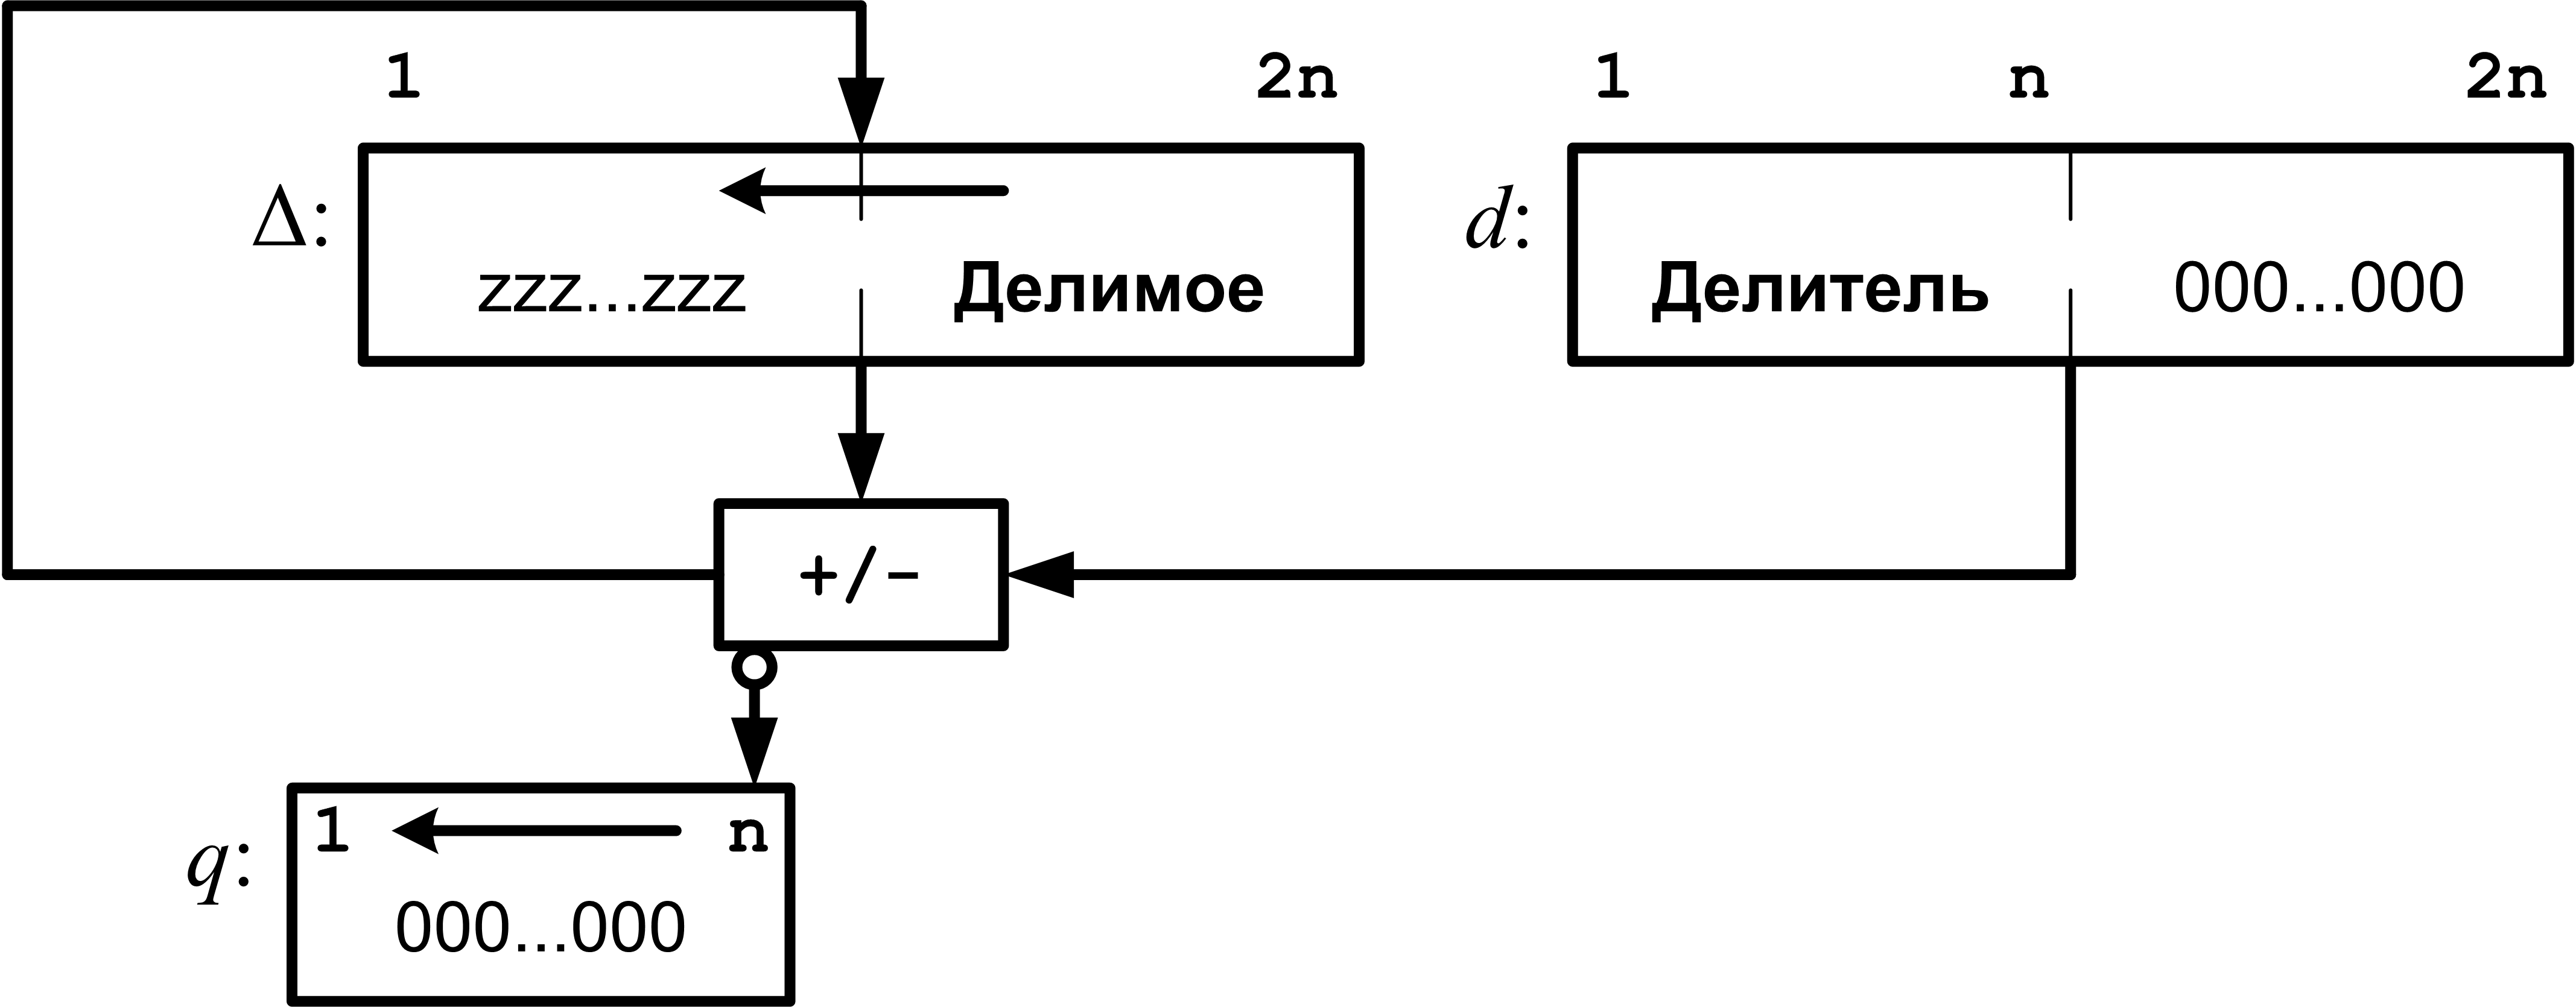
\includegraphics[width=0.47\textwidth]{fig/IDivBegin}
            & 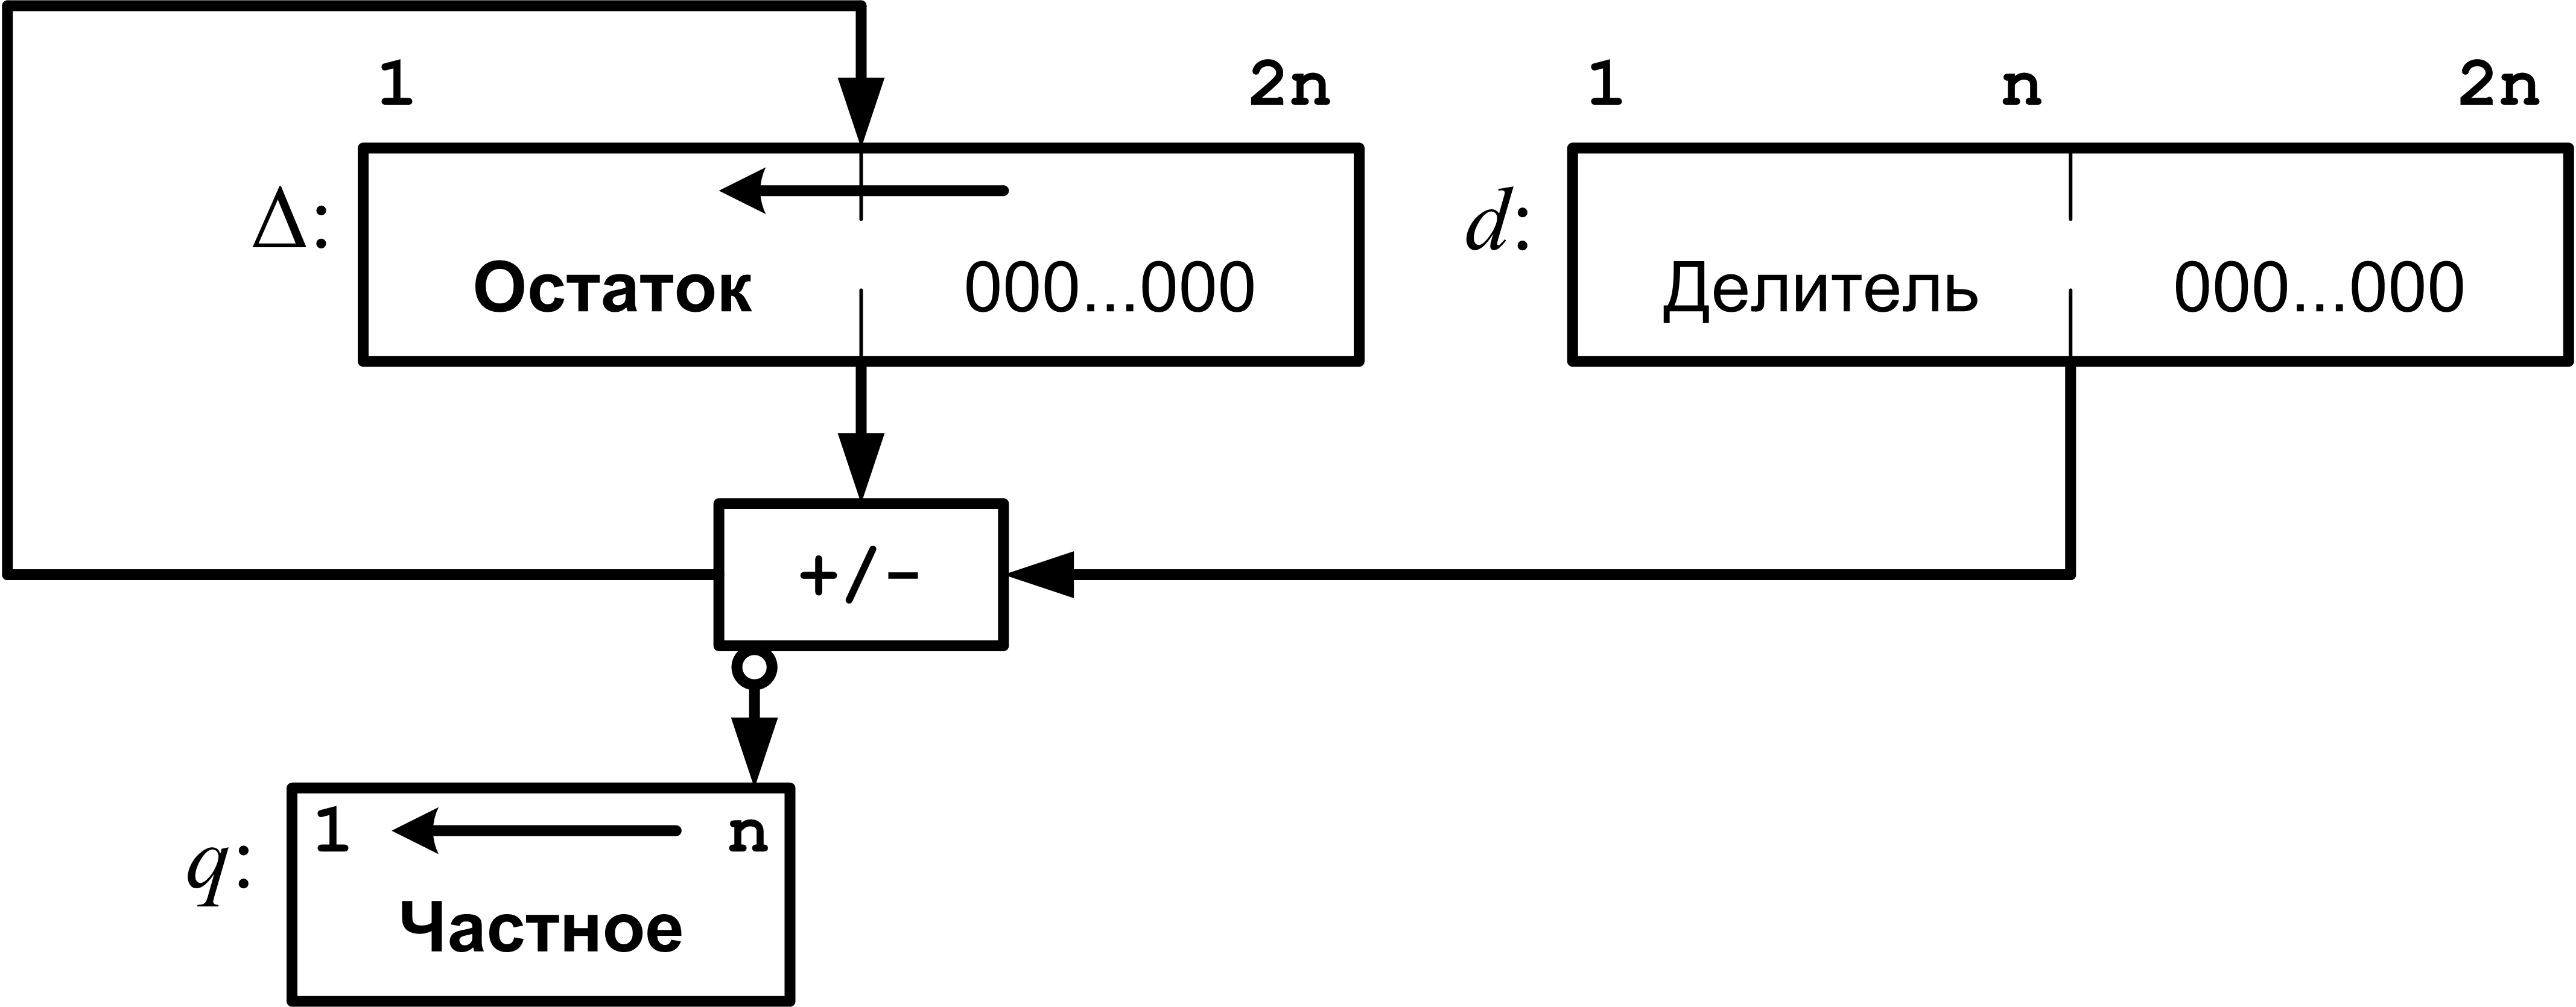
\includegraphics[width=0.47\textwidth]{fig/IDivEnd} \\
        а) начало деления
            & б) конец деления
    \end{tabular}
    \caption{I-й способ целочисленного деления} \label{t:div:int:Isp}
\end{figure}

\begin{figure}[!ht]
    \centering
    \begin{tabular}{c||c}
        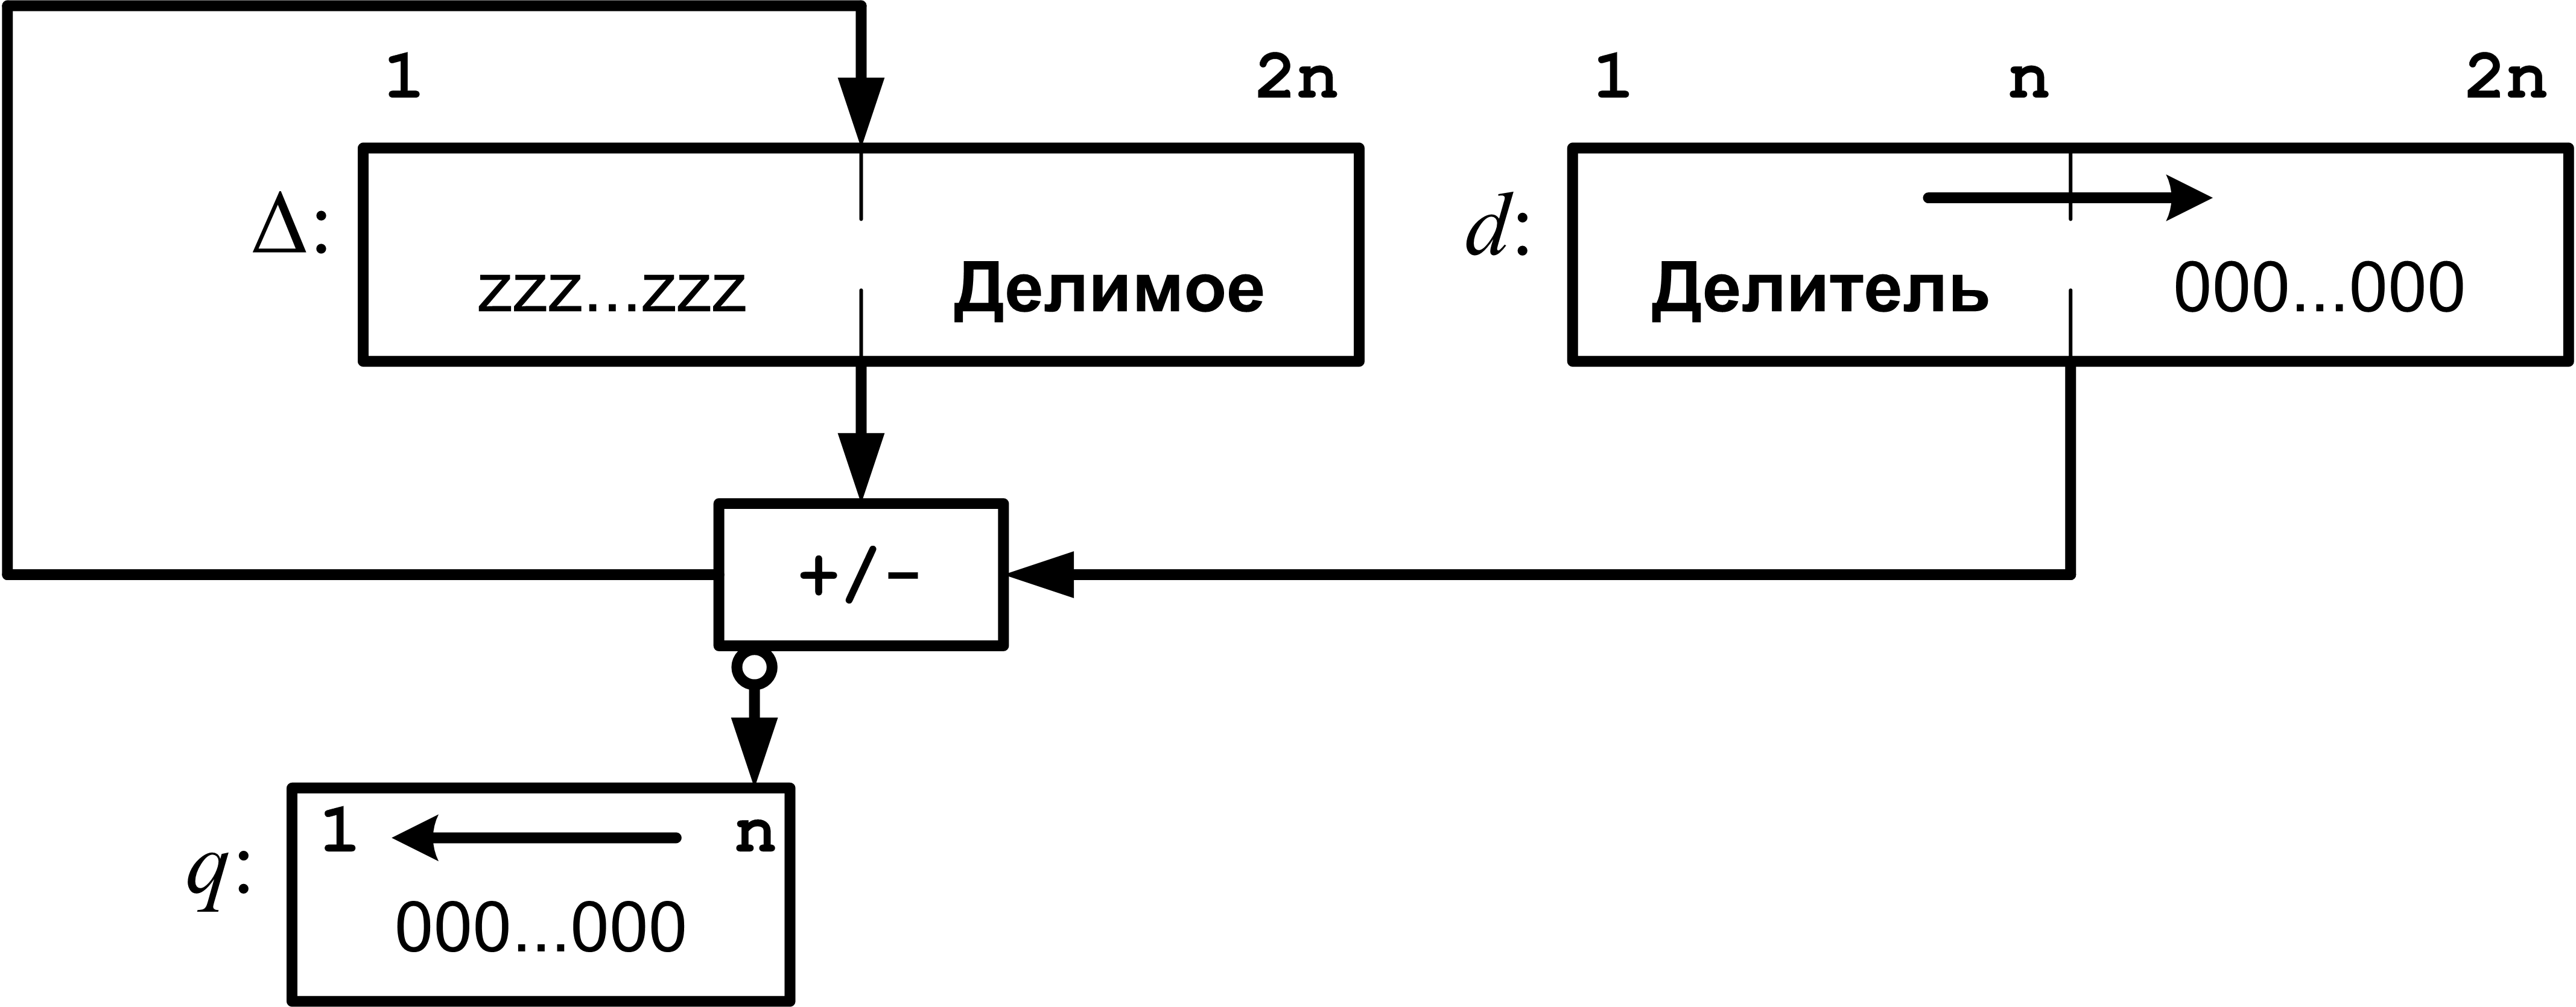
\includegraphics[width=0.47\textwidth]{fig/IIDivBegin}
            & 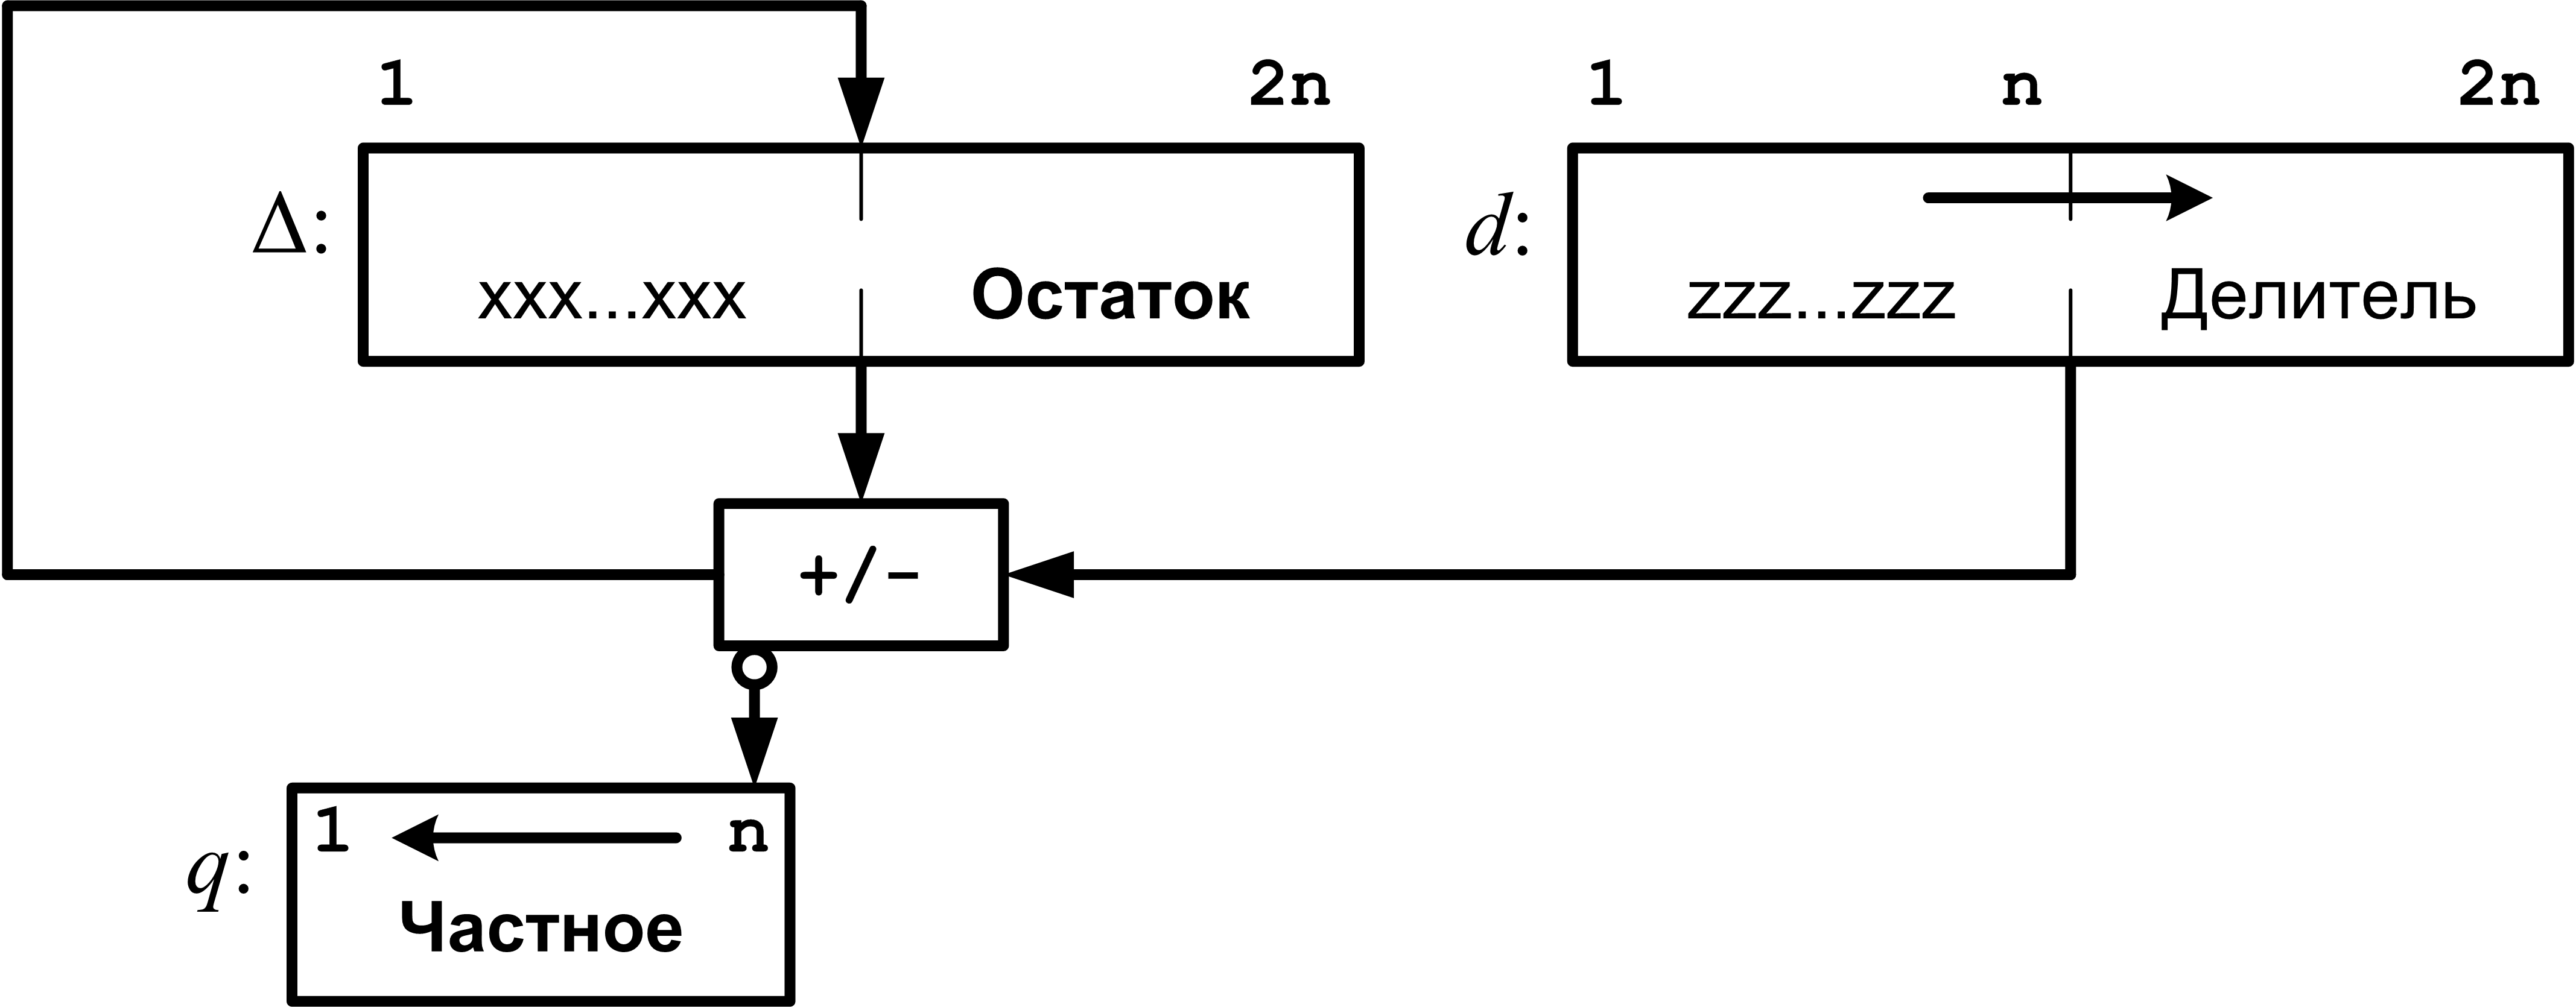
\includegraphics[width=0.47\textwidth]{fig/IIDivEnd} \\
        а) начало деления
            & б) конец деления
    \end{tabular}
    \caption{II-й способ целочисленного деления} \label{t:div:int:IIsp}
\end{figure}

Рассмотрим алгоритм деления с <<Восстановлением остатков>>. Особенностью данного алгоритма является то, что полученная разность регистров остатка $\Delta$ и делителя $d$ (остаток текущего шага) всегда запоминается в регистре остатков (что проще реализовать технически). И если в регистре остатка получено отрицательное значение, то требуется восстановить его положительное значение до вычитания, прибавив делитель.

Алгоритм деления с <<восстановлением остатков>> следующий.
\begin{enumerate}
	\item Если делитель --- ноль, то фиксируется ошибка вычислений и алгоритм завершается.
	\item $i\gets 1$. В младшую часть регистра остатков заносится делимое, в старшую часть регистра делителя --- делитель. Далее состояние регистра остатков --- остаток ($\Delta$), регистра делителя --- делитель ($d$), регистра частного ($q$) --- частное.
	\item\label{e:div:int:vo:start} Выполняются сдвиги: частное $q$ влево, остаток $\Delta$ влево (в первом способе), делитель $d$ вправо (во втором способе).
	\item Получается новый остаток $\Delta\gets(\Delta - d)$;
	\item Если $\Delta < 0$, то в младший разряд частного заносится $0$, иначе $1$.
	\item Если $\Delta < 0$, то выполняется \emph{восстановление} старого значения остатка: $\Delta\gets(\Delta + d)$.
	\item $i\gets (i + 1)$. Если $i\le n$, то к шагу \ref{e:div:int:vo:start}.
	\item В регистре частного получено значение частного, в регистре остатков --- $n$-разрядный остаток (в первом способе в старших разрядах, во втором --- в младших).
\end{enumerate}

Так как в основном цикле алгоритма происходит проверка знака остатка ($\Delta < 0$), то к регистру остатка и делителю добавляется знаковый разряд. Пример деления с восстановлением остатков I-м способом в шестиразрядной сетке приведен на рисунке \ref{t:div:int:IspVoEx}, а II-м --- на рисунке \ref{t:div:int:IIspVoEx}.

\begin{figure}[!ht]
    \centering
	\begin{tabular}{c|r|r|l}
		\hline\hline
		$q, \leftarrow$ 
			& \multicolumn{1}{|c|}{$\Delta, \leftarrow$}
				& \multicolumn{1}{|c|}{$d$}
					& прим.\\ 
		\hline\hline
		\Number{......}
			& \Number{.,...... 111001}
				& \Number{.,...110}
					& исх. операнды;\\ \hline\hline
		\Number{......}
			& \Number{.,.....1 11001.}
				& 
					& сдвиг;\\ \hline
		\Number{.....0}
			& \Addition{.,.....1 11001.}
					   {1,111010 ......}
					   {1,111011 11001.}
				& 
					& $\Delta_1<0$;\\ \hline
		\Number{.....0}
			& \Addition{1,111011 11001.}
					   {.,...110 ......}
					   {.,.....1 11001.}
				& 
					& ВО $\Delta_1$; \\ \hline
		\Number{....0.}
			& \Number{.,....11 1001..}
				& 
					& сдвиг;\\ \hline
		\Number{....00}
			& \Addition{.,....11 1001..}
					   {1,111010 ......}
					   {1,111101 1001..}
				& 
					& $\Delta_2<0$;\\ \hline
		\Number{....00}
			& \Addition{1,111101 1001..}
					   {.,...110 ......}
					   {.,....11 1001..}
				& 
					& ВО $\Delta_2$; \\ \hline
		\Number{...00.}
			& \Number{.,...111 001...}
				& 
					& сдвиг;\\ \hline
		\Number{...001}
			& \Addition{.,...111 001...}
					   {1,111010 ......}
					   {.,.....1 001...}
				& 
					& $\Delta_3> 0$; Без ВО\\ \hline
		\Number{..001.}
			& \Number{.,....10 01....}
				& 
					& сдвиг;\\ \hline
		\Number{..0010}
			& \Addition{.,....10 01....}
					   {1,111010 ......}
					   {1,111100 01....}
				& 
					& $\Delta_4<0$;\\ \hline
		\Number{..0010}
			& \Addition{1,111100 01....}
					   {.,...110 ......}
					   {.,....10 01....}
				& 
					& ВО $\Delta_4$; \\ \hline
		\Number{.0010.}
			& \Number{.,...100 1.....}
				& 
					& сдвиг;\\ \hline
		\Number{.00100}
			& \Addition{.,...100 1.....}
					   {1,111010 ......}
					   {1,111110 1.....}
				& 
					& $\Delta_5<0$;\\ \hline
		\Number{.00100}
			& \Addition{1,111110 1.....}
					   {.,...110 ......}
					   {.,...100 1.....}
				& 
					& ВО $\Delta_5$; \\ \hline
		\Number{00100.}
			& \Number{.,..1001 ......}
				& 
					& сдвиг;\\ \hline
		\Number{001001}
			& \Addition{.,..1001 ......}
					   {1,111010 ......}
					   {0,000011 ......}
				& 
					& $\Delta_6>0$; Без ВО\\ \hline\hline
		\Number{001001}
			& \Number{000011}
				&
					& $\DivAnswer{q}{\Delta_6}$;\\ 
	\end{tabular}
	
    \caption{$57\div 6 = \DivAnswer{9}{1}$ I-сп с восстановлением остатков, $n=6$}
    \label{t:div:int:IspVoEx}
\end{figure}

\begin{figure}[!ht]
    \centering
	\begin{tabular}{c|r|r|l}
		\hline\hline
		$q, \leftarrow$ 
			& \multicolumn{1}{|c|}{$\Delta$}
				& \multicolumn{1}{|c|}{$d,\rightarrow$}
					& прим. \\ 
		\hline\hline
		\Number{......}
			& \Number{.,...... 111110}
				& \Number{.,...110 ......}
					& операнды;\\ \hline\hline
		\Number{......}
			& 
				& \Number{.,....11 0.....}
					& сдвиг;\\ \hline
		\Number{.....0}
			& \Addition{.,...... 111110}
					   {1,111101 0.....}
					   {1,111101 111110}
				& 
					& $\Delta_1<0$;\\ \hline
		\Number{.....0}
			& \Addition{1,111101 111110}
					   {.,....11 0.....}
					   {.,...... 111110}
				& 
					& ВО $\Delta_1$;\\ \hline
		\Number{....0.}
			& 
				& \Number{.,.....1 10....}
					& сдвиг;\\ \hline
		\Number{....00}
			& \Addition{.,...... 111110}
					   {1,111110 10....}
					   {1,111111 011110}
				& 
					& $\Delta_2<0$;\\ \hline
		\Number{....00}
			& \Addition{1,111111 011110}
					   {.,.....1 10....}
					   {.,...... 111110}
				& 
					& ВО $\Delta_2$;\\ \hline
		\Number{...00.}
			& 
				& \Number{.,...... 110...}
					& сдвиг;\\ \hline
		\Number{...001}
			& \Addition{.,...... 111110}
					   {1,111111 010...}
					   {0,000000 001110}
				& 
					& $\Delta_3>0$; Без ВО\\ \hline
		\Number{..001.}
			& 
				& \Number{.,...... .110..}
					& сдвиг;\\ \hline
		\Number{..0010}
			& \Addition{.,...... ..1110}
					   {1,111111 1010..}
					   {1,111111 110110}
				& 
					& $\Delta_4<0$;\\ \hline
		\Number{..0010}
			& \Addition{1,111111 110110}
					   {.,...... .110..}
					   {.,...... ..1110}
				& 
					& ВО $\Delta_4$;\\ \hline
		\Number{.0010.}
			& 
				& \Number{.,...... ..110.}
					& сдвиг;\\ \hline
		\Number{.00101}
			& \Addition{.,...... ..1110}
					   {1,111111 11010.}
					   {0,000000 000010}
				& 
					& $\Delta_5>0$; Без ВО\\ \hline
		\Number{00101.}
			& 
				& \Number{.,...... ...110}
					& сдвиг;\\ \hline
		\Number{001010}
			& \Addition{.,...... ....10}
					   {1,111111 111010}
					   {1,111111 111100}
				& 
					& $\Delta_6<0$;\\ \hline
		\Number{001010}
			& \Addition{1,111111 111100}
					   {.,...... ...110}
					   {.,...... ....10}
				& 
					& ВО $\Delta_6$; \\ \hline\hline
	\Number{001010}
		& \Number{000010}
			&
				& $\DivAnswer{q}{\Delta_6}$;\\ 
	\end{tabular}
		
    \caption{$62\div 6 = \DivAnswer{10}{2}$ II-сп. с восстановлением остатков, $n=6$}
    \label{t:div:int:IIspVoEx}
\end{figure}

Рассмотрим, что произойдет с остатком в изложенном выше алгоритме деления с восстановлением остатков. 
Если новый остаток $\Delta$ получается отрицательным, то к нему прибавляется делитель, чтобы восстановить старое (положительное) значение остатка. Чтобы не тратить на это время (а на восстановление требуется такт) --- проследим, что происходит к моменту получения следующего остатка $\Delta'$.
    
\begin{itemize}
	\item В первом способе: 
	\[
		\Delta' = 
			\begin{cases}
				2\cdot\Delta + d, & \text{ если $\Delta<0$: $2\cdot(\underbrace{\Delta + d}_\text{В.О.}) - d = 2\cdot\Delta + d$,}\\
				2\cdot\Delta - d, & \text{ если $\Delta\ge 0$.}
			\end{cases}
	\]
	
	\item Во втором способе:
	\[
		\Delta' = 
			\begin{cases}
				\Delta + d/2, & \text{ если $\Delta<0$: $(\underbrace{\Delta + d}_\text{В.О.}) - d/2 = \Delta + d/2$,}\\
				\Delta - d/2, & \text{ если $\Delta\ge 0$.}
			\end{cases}
	\]
\end{itemize}

Таким образом, если остаток получается отрицательным, то восстановление не выполняется, а на следующем шаге после соответствующих сдвигов, делитель прибавляется к остатку.

Алгоритм деления без восстановления остатков.
\begin{enumerate}
	\item Если делитель --- ноль, то фиксируется ошибка вычислений и алгоритм завершается.
	\item $i\gets 1$; В младшую часть регистра остатков заносится делимое, в старшую часть регистра делителя --- делитель. Далее состояние регистра остатков --- остаток ($\Delta$), регистра делителя --- делитель ($d$), регистра частного ($q$) --- частное.
	\item\label{div:wvo:start} Выполняются сдвиги: частное $q$ влево, остаток $\Delta$ влево (в первом способе), делитель $d$ вправо (во втором способе).
	\item Если $\Delta < 0$, то $\Delta\gets(\Delta + d)$, иначе $\Delta\gets(\Delta - d)$;
	\item Если $\Delta < 0$, то в младший разряд частного заносится 0, иначе 1.
	\item $i\gets (i + 1)$. Если $\le n$, то к шагу \ref{div:wvo:start}.
	\item Восстанавливается последний остаток. Если $\Delta < 0$, то $\Delta\gets(\Delta + d)$.
	\item В регистре частного получено значение частного, в регистре остатков --- $n$-разрядный остаток (в первом способе в старших разрядах, во втором --- в младших).
\end{enumerate}


На рисунках \ref{t:div:int:IspNoVoEx} и \ref{t:div:int:IIspNoVoEx} приводятся примеры деления без восстановления остатков I и II-м способами соответственно. Сравните результаты с примерами на рисунках \ref{t:div:int:IspVoEx} и \ref{t:div:int:IIspVoEx}.

\begin{figure}[!ht]
    \centering
	\begin{tabular}{c|r|r|l}
		\hline\hline
		$q, \leftarrow$ 
			& \multicolumn{1}{|c|}{$\Delta, \leftarrow$}
				& \multicolumn{1}{|c|}{$d$}
					& прим.\\ 
		\hline\hline
		\Number{......}
			& \Number{.,...... 111001}
				& \Number{.,...110}
					& исх. операнды;\\ \hline\hline
		\Number{......}
			& \Number{.,.....1 11001.}
				& 
					& сдвиг;\\ \hline
		\Number{.....0}
			& \Addition{.,.....1 11001.}
					   {1,111010 ......}
					   {1,111011 11001.}
				& 
					& ${-d},\Delta_1<0$;\\ \hline
		\Number{....0.}
			& \Number{1,110111 1001..}
				& 
					& сдвиг;\\ \hline
		\Number{....00}
			& \Addition{1,110111 1001..}
					   {.,...110 ......}
					   {1,111101 1001..}
				& 
					& ${+d},\Delta_2<0$;\\ \hline
		\Number{...00.}
			& \Number{1,111011 001...}
				& 
					& сдвиг;\\ \hline
		\Number{...001}
			& \Addition{1,111011 001...}
					   {.,...110 ......}
					   {.,.....1 001...}
				& 
					& $\Delta_3> 0$;\\ \hline
		\Number{..001.}
			& \Number{.,....10 01....}
				& 
					& сдвиг;\\ \hline
		\Number{..0010}
			& \Addition{.,....10 01....}
					   {1,111010 ......}
					   {1,111100 01....}
				& 
					& ${-d},\Delta_4<0$;\\ \hline
		\Number{.0010.}
			& \Number{1,111000 1.....}
				& 
					& сдвиг;\\ \hline
		\Number{.00100}
			& \Addition{1,111000 1.....}
					   {.,...110 ......}
					   {1,111110 1.....}
				& 
					& $\Delta_5<0$;\\ \hline
		\Number{00100.}
			& \Number{1,111101 ......}
				& 
					& сдвиг;\\ \hline
		\Number{001001}
			& \Addition{1,111101 ......}
					   {.,...110 ......}
					   {0,000011 ......}
				& 
					& $\Delta_6>0$;\\ \hline\hline
		\Number{001001}
			& \Number{000011}
				&
					& $\DivAnswer{q}{\Delta_6}$;\\ 
	\end{tabular}
	
    \caption{$57\div 6 = \DivAnswer{9}{1}$ I-сп без восстановления остатков, $n=6$}
    \label{t:div:int:IspNoVoEx}
\end{figure}

\begin{figure}[!ht]
    \centering
	\begin{tabular}{c|r|r|l}
		\hline\hline
		$q, \leftarrow$ 
			& \multicolumn{1}{|c|}{$\Delta$}
				& \multicolumn{1}{|c|}{$d,\rightarrow$}
					& прим. \\ 
		\hline\hline
		\Number{......}
			& \Number{.,...... 111110}
				& \Number{.,...110 ......}
					& операнды;\\ \hline\hline
		\Number{......}
			& \Number{.,...... 111110}
				& \Number{.,....11 0.....}
					& сдвиг;\\ \hline
		\Number{.....0}
			& \Addition{.,...... 111110}
					   {1,111101 0.....}
					   {1,111101 111110}
				& 
					& $-d, \Delta_1<0$;\\ \hline
		\Number{....0.}
			& 
				& \Number{.,.....1 10....}
					& сдвиг;\\ \hline
		\Number{....00}
			& \Addition{1,111101 111110}
					   {.,.....1 10....}
					   {1,111111 011110}
				& 
					& $+d, \Delta_2<0$;\\ \hline
		\Number{...00.}
			& 
				& \Number{.,...... 110...}
					& сдвиг;\\ \hline
		\Number{...001}
			& \Addition{1,111111 011110}
					   {.,...... 110...}
					   {.,...... ..1110}
				& 
					& $+d, \Delta_3>0$;\\ \hline
		\Number{..001.}
			& 
				& \Number{.,...... .110..}
					& сдвиг;\\ \hline
		\Number{..0010}
			& \Addition{.,...... ..1110}
					   {1,111111 1010..}
					   {1,111111 110110}
				& 
					& $-d, \Delta_4<0$;\\ \hline
		\Number{.0010.}
			& 
				& \Number{.,...... ..110.}
					& сдвиг;\\ \hline
		\Number{.00101}
			& \Addition{1,111111 110110}
					   {.,...... ..110.}
					   {.,...... ....10}
				& 
					& $+d, \Delta_5>0$;\\ \hline
		\Number{00101.}
			& 
				& \Number{.,...... ...110}
					& сдвиг;\\ \hline
		\Number{001010}
			& \Addition{.,...... ....10}
					   {1,111111 111010}
					   {1,111111 111100}
				& 
					& $-d, \Delta_6<0$;\\ \hline
		\Number{001010}
			& \Addition{1,111111 111100}
					   {.,...... ...110}
					   {.,...... ....10}
				& 
					& ВО!!! $\Delta_6$; \\ \hline\hline
	\Number{001010}
		& \Number{000010}
			&
				& $\DivAnswer{q}{\Delta_6}$;\\ 
	\end{tabular}
		
    \caption{$62\div 6 = \DivAnswer{10}{2}$ II-сп. с восстановлением остатков, $n=6$}
    \label{t:div:int:IIspNoVoEx}
\end{figure}


\subsection{Деление чисел в дополнительном коде}

Пусть $S(x)$ --- функция, возвращающая знак целого числа $x$. При делении чисел со знаком определение очередного разряда частного будет выполняться по следующим правилам.
\begin{enumerate}
	\item\label{en:div:int:rule:mod} Если знаки делимого $A$ и текущего остатка $\Delta$ совпадают ($S(A)=S(\Delta)$), то разряд частного (модуля) $q_0\gets 1$, иначе $q_0\gets 0$. Таким образом находятся, очевидно, разряды модуля частного.
	\item\label{en:div:int:rule:neg} Далее, если $S(A)$ и $S(d)$ различны, то полученный разряд частного следует инвертировать: $q_0\gets(\lnot q_0)$. Так учитывается, что частное должно получиться отрицательным. Строго говоря, так будут получены разряды обратного кода частного.
\end{enumerate}
    
Так как справедливо, что
\[
	(a=b)\Leftrightarrow \lnot(a\oplus b) \Leftrightarrow (1\oplus a\oplus b),
\]
то исходное правило, записанное одной формулой
\[
	q_0\gets\underbrace{
		\underbrace{\lnot(S(A)=S(\Delta))}_{\text{п. \ref{en:div:int:rule:mod}}}\oplus(S(A)\oplus S(d))
	}_{\text{п. \ref{en:div:int:rule:neg}}}
\]
можно значительно упростить:
\begin{align*}
	\lnot(S(A)=S(\Delta))\oplus(S(A)\oplus S(d)) \Leftrightarrow \\
	\Leftrightarrow(1\oplus S(A)\oplus S(\Delta))\oplus (S(A)\oplus S(d)) \Leftrightarrow (1\oplus S(d)\oplus S(\Delta))\Leftrightarrow \\
	\Leftrightarrow\lnot(S(d)\oplus S(\Delta)).
\end{align*}

Алгоритм деления в ДК без восстановления остатков.
\begin{enumerate}
	\item Если делтель --- ноль, то фиксируется ошибка вычислений и алгоритм завершается.
	\item $i\gets 1$. Инициализируются регистры $q$, $\Delta$ и $d$.
	\item\label{div:dcvo:start} Выполняются сдвиги: $q$ --- влево, $\Delta$ --- влево (I сп.), $d$ --- вправо (II~сп., с учётом знака).
	\item Если знаки $\Delta$ и $d$ совпадают, то $\Delta\gets(\Delta - d)$, иначе $\Delta\gets(\Delta + d)$.
	\item $q_0\gets\lnot(S(d)\oplus S(\Delta))$. Т.е. если знаки $d$ и $\Delta$ совпадают, то $q_0\gets 1$, иначе $q_0\gets 0$.
	\item $i\gets (i + 1)$. Если $i<=n$, то к шагу \ref{div:dcvo:start}.
	\item Выполняется процедура коррекции остатка и частного, действия которой в зависимости от знаков делимого и делителя приведены на рисунке \ref{t:div:int:Signed:Correction}.
\end{enumerate}

\begin{figure}[!ht]
    \centering
	\begin{tabular}{c||c|c}
			& $d> 0$
				& $d < 0$\\
		\hline\hline
		\rotatebox{90}{$A\ge 0$}
			& 
			\parbox[c]{.3\textwidth}{
				\begin{align*}
					q&\gets q,\\
					\Delta&\gets 
					\begin{cases}
						(\Delta + d), & \Delta < 0, \\
						\Delta,      &\text{ иначе,}
					\end{cases}
				\end{align*}
			}
				& 
				\parbox[c]{.3\textwidth}{
					\begin{align*}
						q&\gets (q+1),\\
						\Delta&\gets 
						\begin{cases}
							(\Delta - d), & \Delta < 0, \\
							\Delta,       &\text{ иначе,}
						\end{cases}
					\end{align*}
				}
				\\
		\hline
		\rotatebox{90}{$A < 0$}
			& 
			\parbox[c]{.3\textwidth}{
				\begin{align*}
					q&\gets 
					\begin{cases}
						q,      & (\Delta = 0) \lor (\Delta = -d) \\
						(q+1),  &\text{ иначе,}
					\end{cases}
					\\
					\Delta&\gets 
					\begin{cases}
						0,          & (\Delta = 0) \lor (\Delta = -d), \\
						(\Delta-d), & \Delta > 0, \\
						\Delta,     & \text{ иначе,}
					\end{cases}
				\end{align*}
			}
				& 
				\parbox[c]{.3\textwidth}{
					\begin{align*}
						q&\gets 
						\begin{cases}
							q+1, & (\Delta = 0) \lor (\Delta = d), \\
							q,   &\text{ иначе,}
						\end{cases}
						\\
						\Delta&\gets 
						\begin{cases}
							0,        & (\Delta = 0) \lor (\Delta = d), \\
							\Delta+d, & \Delta > 0, \\
							\Delta,   & \text{ иначе.}
						\end{cases}
					\end{align*}
				} \\ 
	\end{tabular}
	
    \caption{Правила заключительной коррекции остатка и частного по правилу отсечения в алгоритме знакового деления}
    \label{t:div:int:Signed:Correction}
\end{figure}

Пример деления чисел со знаком первым способом приведен на рисунке \ref{t:div:int:Signed:I}.

\begin{figure}[!ht]
    \centering
	\begin{tabular}{c|r|r|l}
		\hline\hline
		$q, \leftarrow$ 
			& \multicolumn{1}{|c|}{$\Delta, \leftarrow$}
				& \multicolumn{1}{|c|}{$d$}
					& прим. \\ 
		\hline\hline
		\Number{......}
			& \Number{0,...... 011100}
				& \Number{1,111011}
					& операнды;\\ \hline\hline
		\Number{......}
			& \Number{0,.....0 11100.}
				& 
					& сдвиг;\\ \hline
		\Number{.....1}
			& \Addition{0,.....0 11100.}
					   {1,111011 ......}
					   {1,111011 11100.}
				& 
					& $+d, \Delta_1<0$;\\ \hline
		\Number{....1.}
			& \Number{1,110111 1100..}
				& 
					& сдвиг;\\ \hline
		\Number{....11}
			& \Addition{1,110111 1100..}
					   {.,...101 ......}
					   {1,111100 1100..}
				& 
					& $-d,\Delta_2<0$;\\ \hline
		\Number{...11.}
			& \Number{1,111001 100...}
				& 
					& сдвиг;\\ \hline
		\Number{...111}
			& \Addition{1,111001 100...}
					   {.,...101 ......}
					   {1,111110 100...}
				& 
					& $-d,\Delta_3<0$;\\ \hline
		\Number{..111.}
			& \Number{1,111101 00....}
				& 
					& сдвиг;\\ \hline
		\Number{..1110}
			& \Addition{1,111101 00....}
					   {.,...101 ......}
					   {0,000010 00....}
				& 
					& $-d,\Delta_4>0$;\\ \hline
		\Number{.1110.}
			& \Number{0,000100 0.....}
				& 
					& сдвиг;\\ \hline
		\Number{.11101}
			& \Addition{0,000100 0.....}
					   {1,111011 ......}
					   {1,111111 0.....}
				& 
					& $+d,\Delta_5<0$;\\ \hline
		\Number{11101.}
			& \Number{1,111110 ......}
				& 
					& сдвиг;\\ \hline
		\Number{111010}
			& \Addition{1,111110 ......}
					   {0,000101 ......}
					   {0,000011 ......}
				& 
					& $-d,\Delta_6>0$;\\ \hline\hline
		\Number{111011}
			& \Number{0,000011 ......}
				& 
					& $q\gets(q+1)$;\\ \hline
		\Number{111011}
			& \Number{000011}
				& 
					& Рез-т;\\
	\end{tabular}

    \caption{$28\div{-5} = \DivAnswer{-5}{3}$ I-сп без ВО, $n=6$}
    \label{t:div:int:Signed:I}
\end{figure}
